\section{Стохастический анализ}

    \subsection{Описание изменений}

        Пришло время провести стохастический анализ. В модели появляется слагаемое, которое отвечает за шум. Это слагаемое имеет следующий вид: \(\varepsilon \xi\), где \(\varepsilon\) --- интенсивность шума, а \(\xi\) --- нормальная случайная величина.

        \comment{Надо написать что такое шум в биологическом смысле. Причем для разных шумов будет разный смысл (исходя из того, зачем нам нужен конкретный параметр)}

        \comment{Ну с \(\beta\)-шумом все ясно, меняется численность популяции, \(\alpha\)-шумом меняется enviroment capacity, а аддитивный какой может иметь смысл?}

        В данную модель шум можно внести тремя способами.

        \(\alpha\)-шум: 

        \begin{equation}
            \label{alpha_chaos}
            x_{t + 1} = \frac{(\alpha + \varepsilon \xi) x_t^2}{(\beta + x_t)^6}
        \end{equation}

        \(\beta\)-шум:

        \begin{equation}
            \label{beta_chaos}
            x_{t + 1} = \frac{\alpha x_t^2}{(\beta + \varepsilon \xi + x_t)^6}
        \end{equation}

        Аддитивный шум:

        \begin{equation}
            \label{additive_chaos}
            x_{t + 1} = \frac{\alpha x_t^2}{(\beta + x_t)^6} + \varepsilon \xi
        \end{equation}

    \subsection{Временные ряды}

        С помощью временных рядов продемонстрируем как различные виды шума влияют на поведение системы. Рассмотрим сразу все возможные варианты шума. 

        На рисунке (\ref{time_series_x_0_06_a_1_b_0_56}) изображено поведение модели без добавления каких-либо шумов. Мы видим, что значения с теченеием времени стабилизируются. Численность популяции фактически осатется неизменной на протяжении всего оставшегося времени.

        \begin{figure}
            \centering
            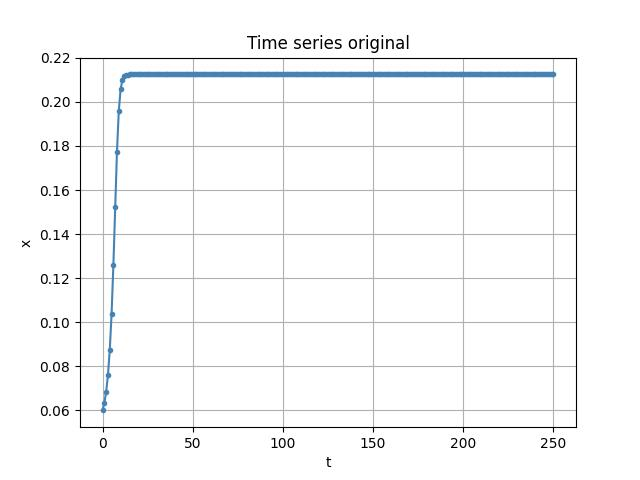
\includegraphics[width=\textwidth]{stochastic/time_series_x_0_06_a_1_b_0_56.jpg}

            \captionsetup{justification=centering}
            \caption{Временной ряд модели (\ref{origin}) при \(\beta = 0.56, \alpha = 1, x_0 = 0.06\)}
            \label{time_series_x_0_06_a_1_b_0_56}
        \end{figure}

        Теперь давайте добавим \(\alpha\)-шум, \(\beta\)-шум, аддитивный шум и рассмотрим соответсвенно рисунки (\ref{time_series_x_0_06_a_1_b_0_56_alpha_chaos_epsilon_0_004}), (\ref{time_series_x_0_06_a_1_b_0_56_beta_chaos_epsilon_0_004}) и ()\(\ref{time_series_x_0_06_a_1_b_0_56_additive_chaos_epsilon_0_004}\)). Все варианты рассматриваются с одной и той же интенсивностью шума \(\varepsilon = 0.004\). Мы видим, что различные виды шума при одинаковой интенсивности влиют на разброс значений в численности популяции. И если раньше численность популяции стабилизировалась и переставала меняться, то сейчас же численность постоянно меняется, но как можно заметить, она меняется в рамках некоторого коридора значений. Численность популяции в общем то не растет и не уменьшается на какую-то значительную величину. Но такое поведение наблюдается не всегда.

        \begin{figure}
            \centering
            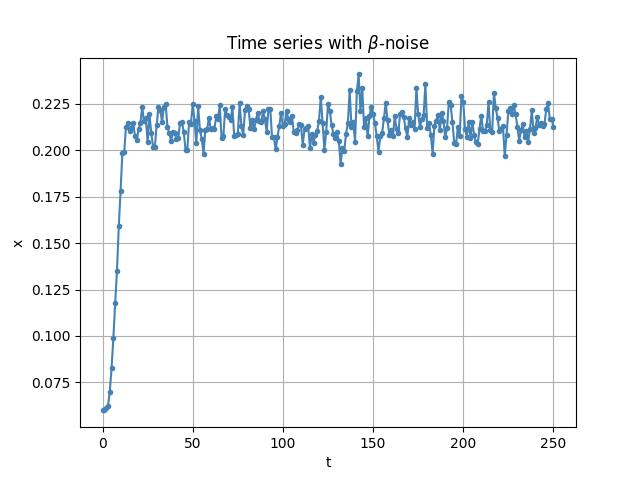
\includegraphics[width=\textwidth]{stochastic/time_series_x_0_06_a_1_b_0_56_beta_chaos_epsilon_0_004.jpg}
        
            \captionsetup{justification=centering}
            \caption{Временной ряд модели (\ref{origin}) при \(\beta = 0.56, \alpha = 1, x_0 = 0.06, \varepsilon = 0.004\)}
            \label{time_series_x_0_06_a_1_b_0_56_beta_chaos_epsilon_0_004}
        \end{figure}

        \begin{figure}
            \centering
            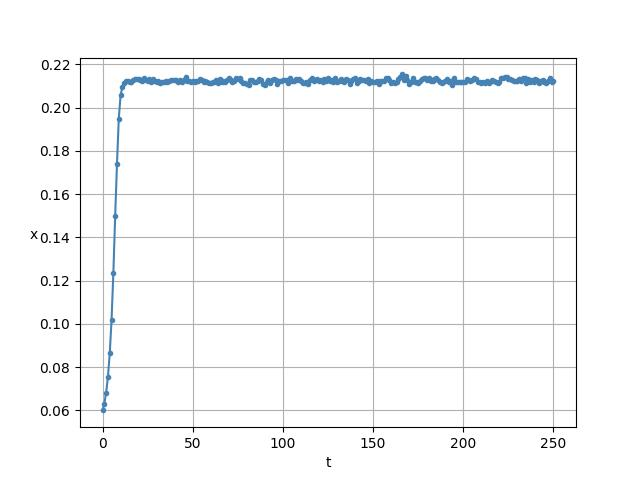
\includegraphics[width=\textwidth]{stochastic/time_series_x_0_06_a_1_b_0_56_alpha_chaos_epsilon_0_004.jpg}
        
            \captionsetup{justification=centering}
            \caption{Временной ряд модели (\ref{origin}) при \(\beta = 0.56, \alpha = 1, x_0 = 0.06, \varepsilon = 0.004\)}
            \label{time_series_x_0_06_a_1_b_0_56_alpha_chaos_epsilon_0_004}
        \end{figure}

        \begin{figure}
            \centering
            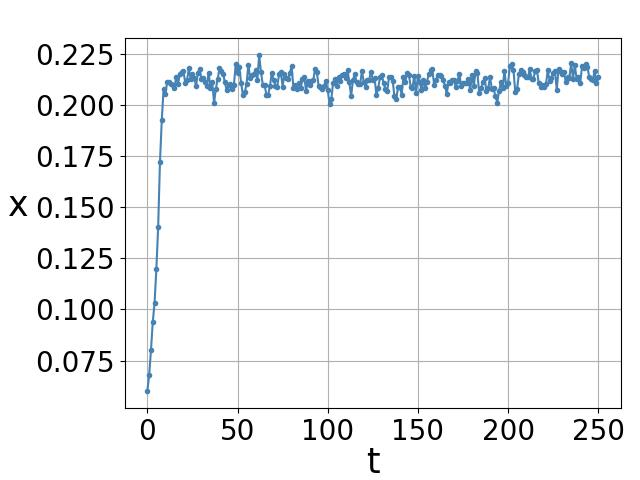
\includegraphics[width=\textwidth]{stochastic/time_series_x_0_06_a_1_b_0_56_additive_chaos_epsilon_0_004.jpg}
        
            \captionsetup{justification=centering}
            \caption{Временной ряд модели (\ref{origin}) при \(\beta = 0.56, \alpha = 1, x_0 = 0.06, \varepsilon = 0.004\)}
            \label{time_series_x_0_06_a_1_b_0_56_additive_chaos_epsilon_0_004}
        \end{figure}

        Для того чтоб продемонстрировать другое возможное поведение, давайте увеличим интенсивность шума. Пускай \(\varepsilon = 0.04\). Рассмотрим рисунок (\ref{time_series_x_0_06_a_1_b_0_56_beta_chaos_epsilon_0_04_fall}). Здесь мы можем увидеть ситуацию, когда шум оказал негативное влияние на то, как меняется численность популяции. Произошло вымирание. Но опять же все не так просто. Если мы еще раз запустим алгоритм, который просчитывает нашу модель, то на картинке (\ref{time_series_x_0_06_a_1_b_0_56_beta_chaos_epsilon_0_04_alive}) увидим, что популяции удалось выжить. Аналогичные эффекты можно наблюдать при других видах шума.

        \begin{figure}
            \centering
            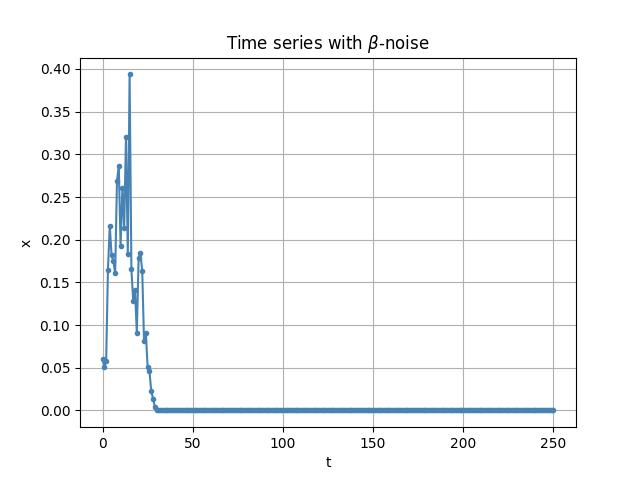
\includegraphics[width=\textwidth]{stochastic/time_series_x_0_06_a_1_b_0_56_beta_chaos_epsilon_0_04_fall.jpg}
        
            \captionsetup{justification=centering}
            \caption{Временной ряд модели (\ref{origin}) при \(\beta = 0.56, \alpha = 1, x_0 = 0.06, \varepsilon = 0.04\)}
            \label{time_series_x_0_06_a_1_b_0_56_beta_chaos_epsilon_0_04_fall}
        \end{figure}

        \begin{figure}
            \centering
            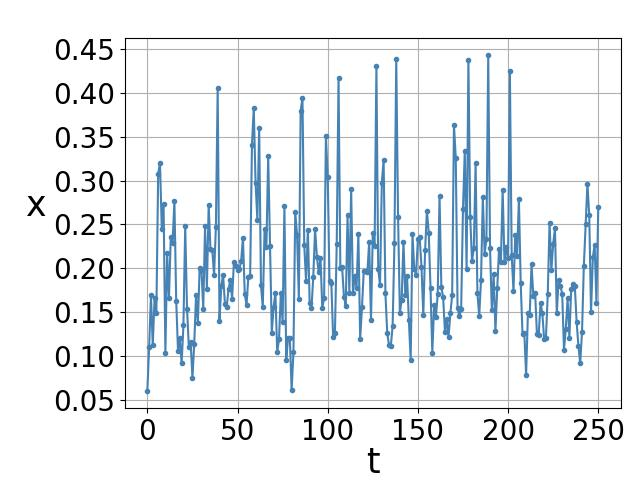
\includegraphics[width=\textwidth]{stochastic/time_series_x_0_06_a_1_b_0_56_beta_chaos_epsilon_0_04_alive.jpg}
        
            \captionsetup{justification=centering}
            \caption{Временной ряд модели (\ref{origin}) при \(\beta = 0.56, \alpha = 1, x_0 = 0.06, \varepsilon = 0.04\)}
            \label{time_series_x_0_06_a_1_b_0_56_beta_chaos_epsilon_0_04_alive}
        \end{figure}

        Анализируя вышесказанное можно сказать, что при добавлении в модель случайных событий ее поведение становится непредсказуемым. Одно незначительное измненеие может кардинально повлиять на ход развития событий. 

        "Одно рисовое зернышко может склонить чашу весов" (с) какой-то мультик.

        \comment{рассматривать как в том семестре все возможные варианты поведения системы в зависимости от начальной точки думаю не надо}

    \subsection{Бифуркация}

        Рассмотрим графики бифуркации с разными видами шумов.

        \begin{figure}
            \centering
            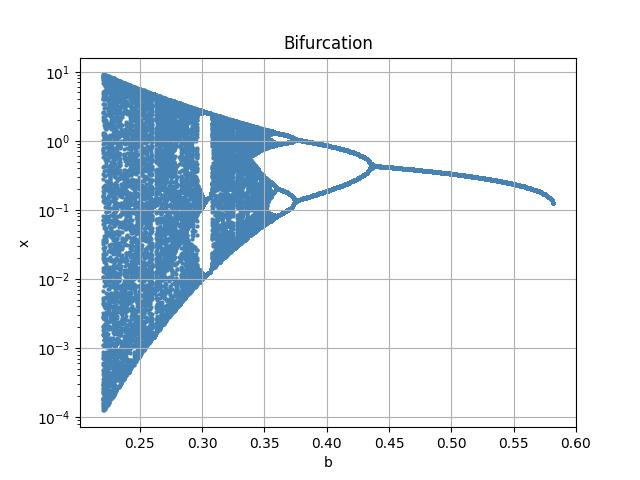
\includegraphics[width=\textwidth]{stochastic/bifurcation_x_0_2_a_1_compare_no_noise.jpg}
        
            \captionsetup{justification=centering}
            \caption{График бифуркации без шума}
            \label{bifurcation_x_0_2_a_1_compare_no_noise}
        \end{figure}

        \begin{figure}
            \centering
            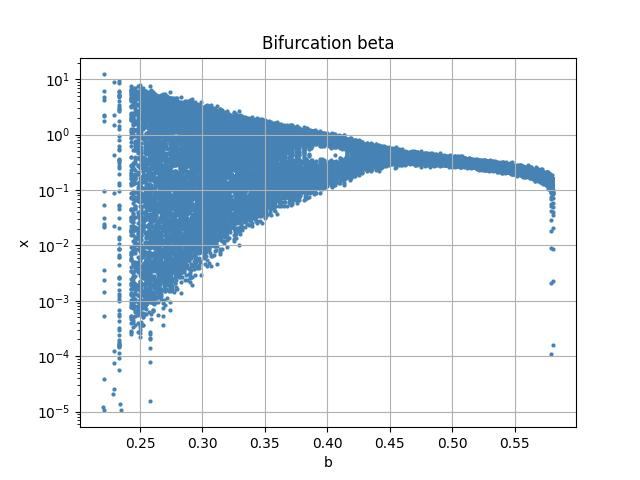
\includegraphics[width=\textwidth]{stochastic/bifurcation_x_0_2_a_1_compare_beta_noise.jpg}
        
            \captionsetup{justification=centering}
            \caption{График бифуркации с \(\beta\)-шумом, \(\varepsilon = 0.01\)}
            \label{bifurcation_x_0_2_a_1_compare_beta_noise}
        \end{figure}

        \begin{figure}
            \centering
            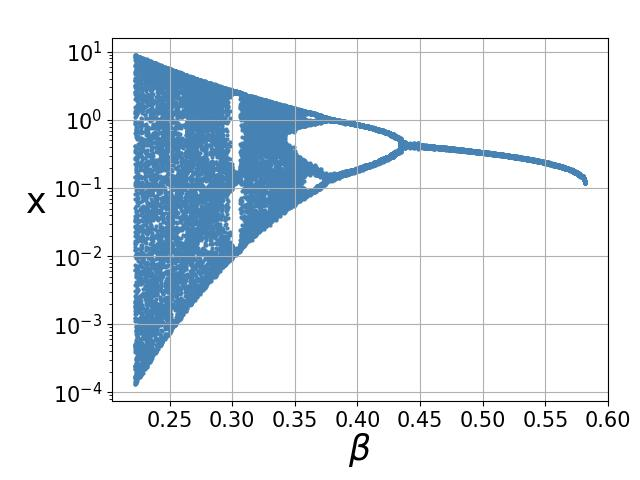
\includegraphics[width=\textwidth]{stochastic/bifurcation_x_0_2_a_1_compare_alpha_noise.jpg}
        
            \captionsetup{justification=centering}
            \caption{График бифуркации с \(\alpha\)-шумом, \(\varepsilon = 0.01\)}
            \label{bifurcation_x_0_2_a_1_compare_alpha_noise}
        \end{figure}

        \begin{figure}
            \centering
            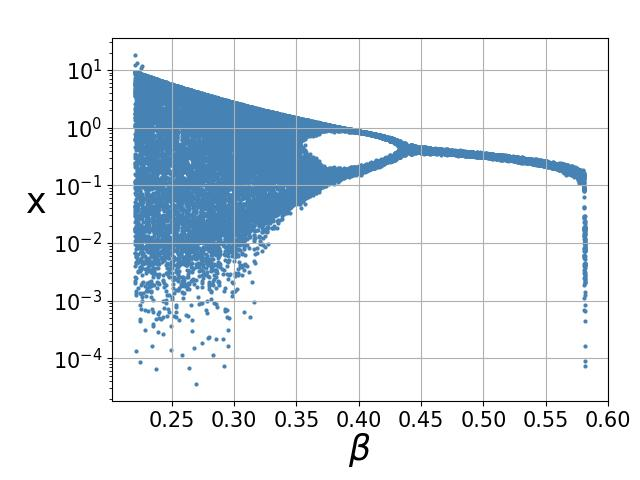
\includegraphics[width=\textwidth]{stochastic/bifurcation_x_0_2_a_1_compare_additional_noise.jpg}
        
            \captionsetup{justification=centering}
            \caption{График бифуркации с аддитивным шумом, \(\varepsilon - 0.01\)}
            \label{bifurcation_x_0_2_a_1_compare_additional_noise}
        \end{figure}

        \comment{напиши что-нибдь про бифуркацю}

    \subsection{Матожидание}

        \comment{напиши что-нибдь про матожидание и циклическое матожидание}

    \subsection{Дисперсия}

        \comment{напиши что-нибдь про дисперсию и циклическую дисперсию}

    \subsection{ФСЧ}
    
        Чтож, а на десерт у нас функция стохастический чувствительности.

        Функция стохастический чувствительности это инструмент, который показывает... Если интересны математические подробности --- иди в статью Crises, noise, and tipping in the Hassell population model.

        Итак, давайте наконец займемся фсч. 

        Давайте посмотрим на график (\ref{bifurcation_x_0_2_a_1_beta_chaos_fss}). Красными линиями нарисована функция стохастический чувствительности. \comment{сформулируй зачем она тут вообще нужна}. 

        У нас есть участок равновесия от \(\beta_i = ...\) до \(\beta_j = ...\) \comment{посмотри выше, там где-то было}. Рассмотрим поближе участок от \(\beta = 0.45\) до \(\beta = 0.48\) на рисунке (\ref{bifurcation_x_0_2_a_1_beta_chaos_fss_segment_stable}). На нем мы видим, что зачения графика бифуркации почти всегда находятся в коридоре ограниченном значенями ФСЧ. Значения высчитваются как \(\pm 3 \sigma\), такой подход по правилу трех сигм гарантирует, что почти все значения будут находится в этом интервале, собственно это мы и наблюдаем.

        На участках с k-циклами и хаосом (\ref{bifurcation_x_0_2_a_1_beta_chaos_fss_segment_2_cycle}), (\ref{bifurcation_x_0_2_a_1_beta_chaos_fss_segment_chaos_down}) и (\ref{bifurcation_x_0_2_a_1_beta_chaos_fss_segment_chaos_up]}) будет наблюдаться аналогичная ситуация. 

        \begin{figure}
            \centering
            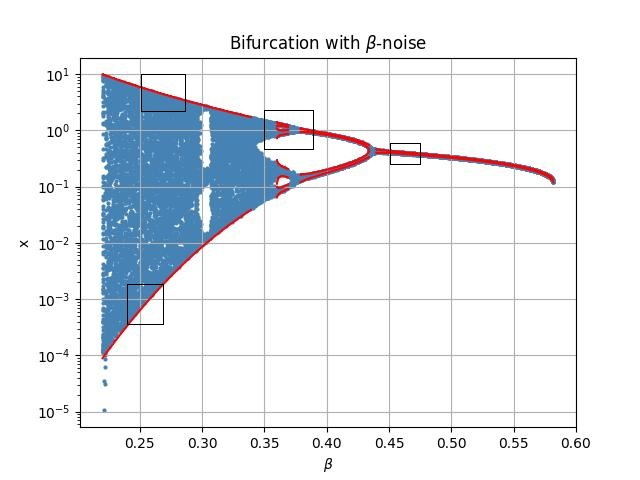
\includegraphics[width=\textwidth]{stochastic/bifurcation_x_0_2_a_1_beta_noise_fss.jpg}
        
            \captionsetup{justification=centering}
            \caption{График бифуркации с \(\beta\)-шумом.}
            \label{bifurcation_x_0_2_a_1_beta_chaos_fss}
        \end{figure}

        \begin{figure}
            \centering
            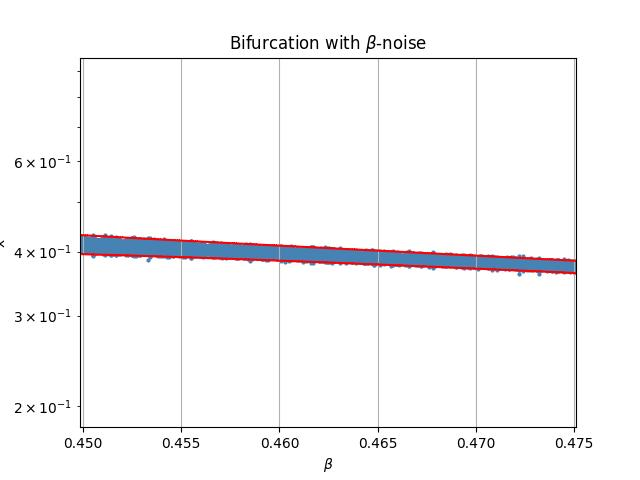
\includegraphics[width=\textwidth]{stochastic/bifurcation_x_0_2_a_1_beta_noise_fss_segment_stable.jpg}
        
            \captionsetup{justification=centering}
            \caption{}
            \label{bifurcation_x_0_2_a_1_beta_chaos_fss_segment_stable}
        \end{figure}

        \begin{figure}
            \centering
            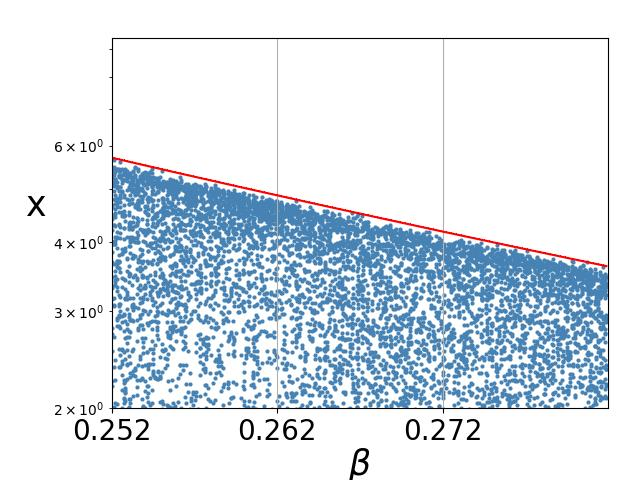
\includegraphics[width=\textwidth]{stochastic/bifurcation_x_0_2_a_1_beta_noise_fss_segment_chaos_up.jpg}
        
            \captionsetup{justification=centering}
            \caption{}
            \label{bifurcation_x_0_2_a_1_beta_chaos_fss_segment_chaos_up}
        \end{figure}

        \begin{figure}
            \centering
            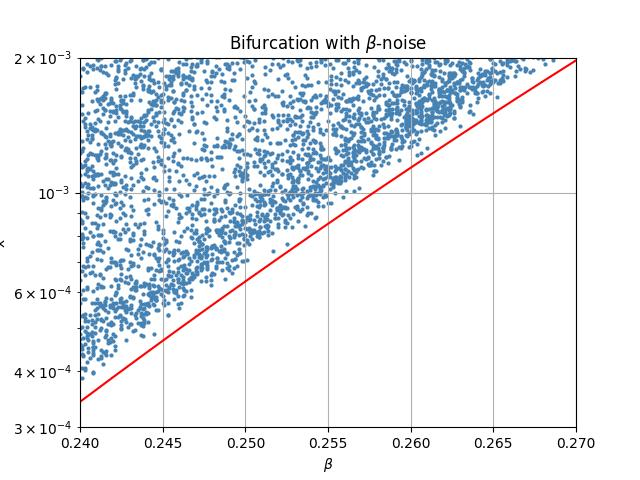
\includegraphics[width=\textwidth]{stochastic/bifurcation_x_0_2_a_1_beta_noise_fss_segment_chaos_down.jpg}
        
            \captionsetup{justification=centering}
            \caption{}
            \label{bifurcation_x_0_2_a_1_beta_chaos_fss_segment_chaos_down}
        \end{figure}

        \begin{figure}
            \centering
            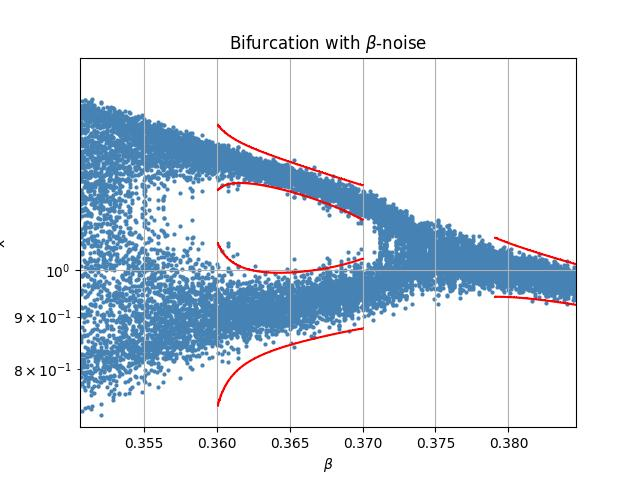
\includegraphics[width=\textwidth]{stochastic/bifurcation_x_0_2_a_1_beta_noise_fss_segment_2_cycle.jpg}
        
            \captionsetup{justification=centering}
            \caption{}
            \label{bifurcation_x_0_2_a_1_beta_chaos_fss_segment_2_cycle}
        \end{figure}

        \comment{напиши что-нибдь про ФСЧ}

    \subsection{График ФСЧ}

        \comment{напиши что-нибдь про график фсч}
        